% Figure: symmetric fixed points of the frozen-calibration mean field of attention and learning at the base point
% (F = 0.99, Q = 1 - F^2, sigma_s^2 = 1, sigma_c^2 = 0.05, n = 4, kappa = 3, vartheta = pi/2, alpha = 0.1, h = 0.995),
% thm:frm-formation, obs:frm-thresholds, tab:frm-thresholds. Computed with the exact set softmax over the 35
% attended sets and the split calibration sigma_in^2 = 0.29872, D_cal = 1.24123, Lambda_0 = 20.0646, p* = 0.0503.
% For each bias fraction x the cross attention P(x; gamma) falls strictly in gamma, so the symmetric fixed points
% are the curve gamma(x) solving x P(x; gamma) = p*(1 - x). Stability from the symmetric and symmetry-breaking
% multipliers of thm:frm-formation(d): stable for gamma < 87.92 on the merged branch (symmetry-breaking multiplier
% reaches one at x = 0.1324), folds at gamma = 105.89 (x = 0.1691) and 60.053 (x = 0.6318), split branch stable
% from gamma = 60.111 (x = 0.6551). Fixed points 0.1129 (gamma = 40), 0.1187 (60) and 0.1274, 0.2999, 0.9659 (80)
% as in tab:frm-thresholds. Thresholds gamma_M = 6.845, gamma_S = 68.15; conditions (i), (ii) of
% thm:frm-formation(b) fail at gamma = 240 and hold at 244. Bridged states (stable per-receiver fixed points with
% 1 to 3 of the 4 cross edges learned) found by continuation: three learned edges from gamma = 43.41 (fold) to
% 111.0, two from 46.69 to 151.0, one from 51.55 to the fold at 240.98; union 43.4 < gamma < 241.0 (shaded).
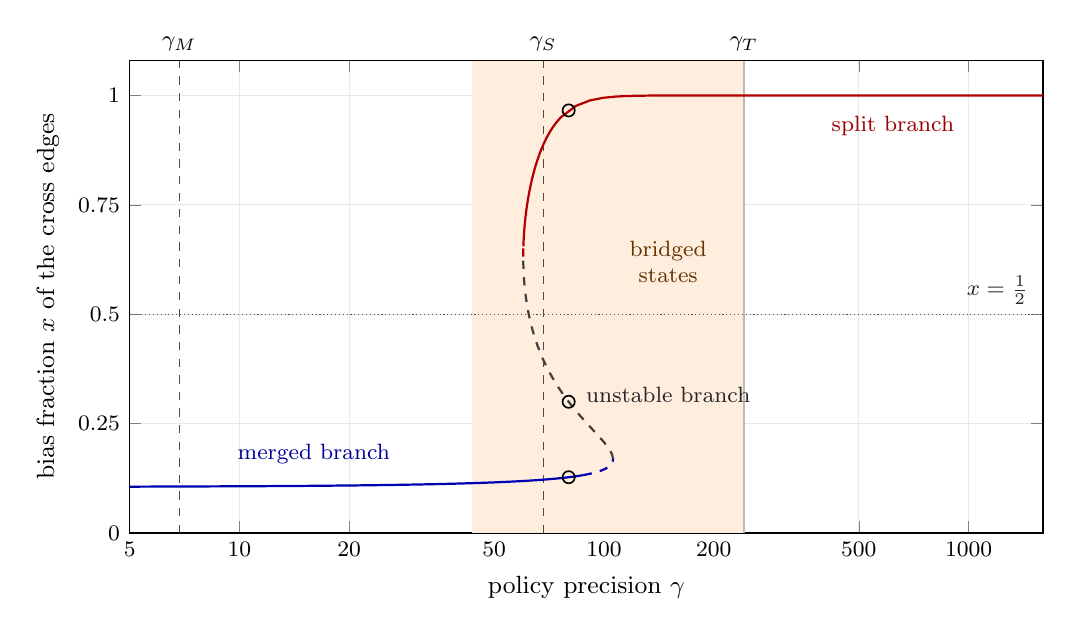
\begin{tikzpicture}
  \begin{axis}[width=11.6cm, height=6.0cm, scale only axis, xmode=log, xmin=5, xmax=1600, ymin=0, ymax=1.08,
      xtick={5,10,20,50,100,200,500,1000}, xticklabels={5,10,20,50,100,200,500,1000}, ytick={0,0.25,0.5,0.75,1},
      grid=major, grid style={gray!18},
      xlabel={policy precision $\gamma$}, ylabel={bias fraction $x$ of the cross edges},
      every axis label/.style={font=\small}, tick label style={font=\footnotesize}, clip=false]
    \fill[orange!13] (axis cs:43.41,0) rectangle (axis cs:240.98,1.08);
    \fill[gray!55] (axis cs:240,0) rectangle (axis cs:244,1.08);
    \draw[gray!60!black, dashed] (axis cs:6.845,0) -- (axis cs:6.845,1.08);
    \draw[gray!60!black, dashed] (axis cs:68.15,0) -- (axis cs:68.15,1.08);
    \draw[gray!60!black, densely dotted] (axis cs:5,0.5) -- (axis cs:1600,0.5);
    \addplot[blue!70!black, thick] coordinates {(5,0.10577) (10.707,0.10676) (16.108,0.10775) (21.22,0.10873) (26.06,0.10972) (30.643,0.11071) (34.983,0.1117) (39.094,0.11268) (42.988,0.11367) (46.677,0.11466) (50.172,0.11565) (53.483,0.11664) (56.621,0.11762) (59.593,0.11861) (62.409,0.1196) (65.078,0.12059) (67.605,0.12157) (70,0.12256) (72.267,0.12355) (74.415,0.12454) (76.448,0.12552) (78.373,0.12651) (80.194,0.1275) (81.917,0.12849) (83.548,0.12948) (85.089,0.13046) (86.546,0.13145) (87.922,0.13244)};
    \addplot[blue!70!black, thick, dashed] coordinates {(87.922,0.13244) (91.439,0.13526) (94.413,0.13807) (96.913,0.14089) (99,0.14371) (100.73,0.14652) (102.13,0.14934) (103.27,0.15216) (104.16,0.15497) (104.83,0.15779) (105.32,0.16061) (105.65,0.16342) (105.83,0.16624) (105.89,0.16906)};
    \addplot[gray!50!black, thick, dashed] coordinates {(105.89,0.16906) (105.31,0.1789) (103.89,0.18875) (101.97,0.19859) (99.765,0.20844) (97.425,0.21828) (95.046,0.22813) (92.692,0.23797) (90.401,0.24782) (88.201,0.25767) (86.103,0.26751) (84.117,0.27736) (82.244,0.2872) (80.484,0.29705) (78.834,0.30689) (77.291,0.31674) (75.849,0.32658) (74.504,0.33643) (73.251,0.34627) (72.084,0.35612) (70.998,0.36596) (69.989,0.37581) (69.051,0.38565) (68.18,0.3955) (67.373,0.40534) (66.625,0.41519) (65.932,0.42503) (65.292,0.43488) (64.701,0.44473) (64.156,0.45457) (63.655,0.46442) (63.195,0.47426) (62.774,0.48411) (62.39,0.49395) (62.041,0.5038) (61.725,0.51364) (61.441,0.52349) (61.187,0.53333) (60.961,0.54318) (60.763,0.55302) (60.591,0.56287) (60.445,0.57271) (60.323,0.58256) (60.224,0.5924) (60.149,0.60225) (60.095,0.6121) (60.064,0.62194) (60.053,0.63179)};
    \addplot[red!70!black, thick, dashed] coordinates {(60.053,0.63179) (60.057,0.63761) (60.068,0.64343) (60.086,0.64925) (60.111,0.65507)};
    \addplot[red!70!black, thick] coordinates {(60.111,0.65507) (60.183,0.66686) (60.284,0.67866) (60.414,0.69046) (60.573,0.70225) (60.762,0.71405) (60.98,0.72585) (61.229,0.73765) (61.51,0.74944) (61.824,0.76124) (62.173,0.77304) (62.559,0.78484) (62.986,0.79663) (63.455,0.80843) (63.971,0.82023) (64.539,0.83203) (65.165,0.84382) (65.858,0.85562) (66.626,0.86742) (67.483,0.87922) (68.445,0.89101) (69.536,0.90281) (70.786,0.91461) (72.244,0.92641) (73.978,0.9382) (76.107,0.95) (83.76,0.9763) (91.55,0.98877) (99.412,0.99467) (107.32,0.99748) (115.24,0.9988) (123.18,0.99943) (131.12,0.99973) (139.07,0.99987) (147.02,0.99994) (154.97,0.99997) (162.92,0.99999) (170.87,0.99999) (178.82,1) (186.77,1) (194.72,1) (202.67,1) (210.62,1) (218.57,1) (226.52,1) (234.47,1) (242.42,1) (250.37,1) (258.32,1) (266.27,1) (274.22,1) (282.17,1) (290.12,1) (298.08,1) (306.03,1) (313.98,1) (321.93,1) (329.88,1) (337.83,1) (371.61,1) (457.79,1) (563.95,1) (694.73,1) (855.84,1) (1054.3,1) (1298.8,1) (1600,1)};
    \addplot[only marks, mark=o, mark size=2.2pt, black, semithick] coordinates {(80,0.1274) (80,0.2999) (80,0.9659)};
    \node[font=\footnotesize, anchor=south] at (axis cs:6.845,1.08) {$\gamma_M$};
    \node[font=\footnotesize, anchor=south] at (axis cs:68.15,1.08) {$\gamma_S$};
    \node[font=\footnotesize, anchor=south] at (axis cs:242,1.08) {$\gamma_T$};
    \node[font=\footnotesize, blue!60!black, anchor=south] at (axis cs:16,0.135) {merged branch};
    \node[font=\footnotesize, red!60!black, anchor=north] at (axis cs:620,0.975) {split branch};
    \node[font=\footnotesize, gray!30!black, anchor=west] at (axis cs:84,0.315) {unstable branch};
    \node[font=\footnotesize, orange!40!black, align=center] at (axis cs:150,0.62) {bridged\\states};
    \node[font=\footnotesize, gray!30!black, anchor=south east] at (axis cs:1550,0.5) {$x=\frac12$};
  \end{axis}
\end{tikzpicture}
